% Created 2022-07-18 Mon 14:33
% Intended LaTeX compiler: pdflatex
\documentclass[11pt]{article}
\usepackage[utf8]{inputenc}
\usepackage[T1]{fontenc}
\usepackage{graphicx}
\usepackage{grffile}
\usepackage{longtable}
\usepackage{rotating}
\usepackage[normalem]{ulem}
\usepackage{amsmath}
\usepackage{textcomp}
\usepackage{amssymb}
\date{\today}
\title{Parallel Robotics Capstone}
\begin{document}

\maketitle
\tableofcontents


\section{Applications}
\label{sec:orge97f799}

\subsection{Why would you even want to do this?}
\label{sec:org750a40a}

\begin{itemize}
\item Two classes of robots
\end{itemize}

\subsubsection{serial (like an arm)}
\label{sec:org6acf918}

\begin{itemize}
\item positioning error is cumumlative
\item long, complex chain structures
\item rigidity decreases as chain count increases
\item joint flexibility dependent on upstream and downstream joints
\end{itemize}

\subsubsection{parallel (like a spider)}
\label{sec:orge50dc6b}

\begin{itemize}
\item each chain relatively short and simple in structure
\item resists unnecessary movement
\item chain positioning error is average
\item off-axis flexibility of joints also affected by other chains
\item provides closed-loop stiffness, robot is rigid relative to components
\item rigidity increases as chain count increases
\end{itemize}

\subsection{Who even does this?}
\label{sec:org94c303a}

Anyone who needs really high precision, has comparably small manipulated objects, and is okay with one location


\subsubsection{Warehousing}
\label{sec:orgeb9c583}

\href{https://www.youtube.com/watch?v=2b4YwFZhtIE}{CoGiRo}

\begin{center}
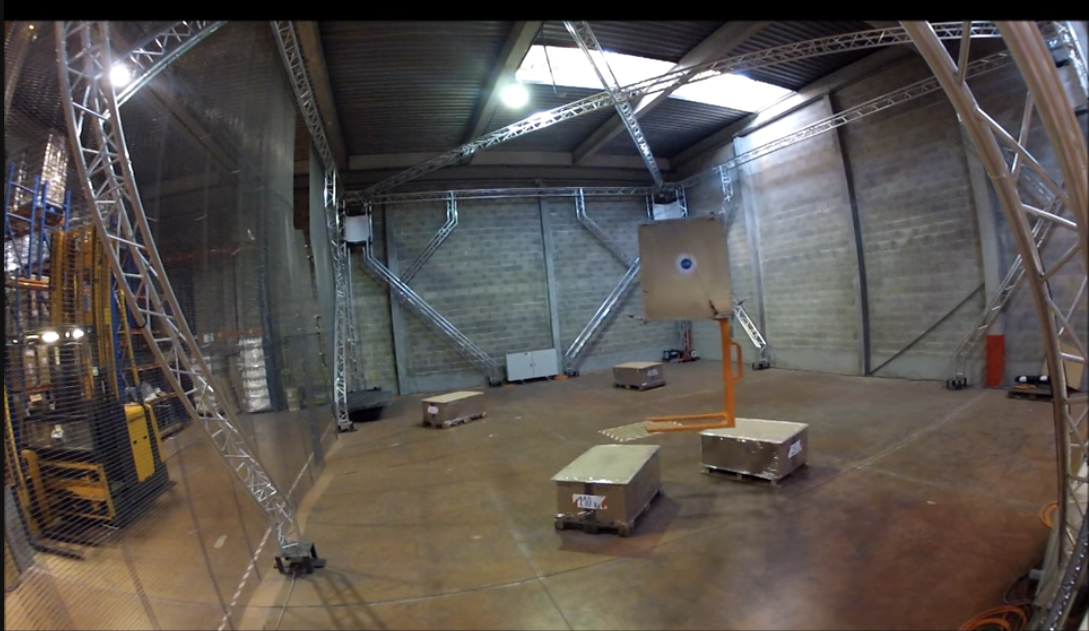
\includegraphics[width=.9\linewidth]{Applications/2022-07-18_12-43-16_screenshot.png}
\end{center}

\subsubsection{Pick + Place + small object manip}
\label{sec:orgdbc0c7f}

Easier + More precise control important/cheaper for small items

\href{https://www.youtube.com/watch?v=QFZMhsVn\_CE}{Pick and Place (China)}

\begin{center}
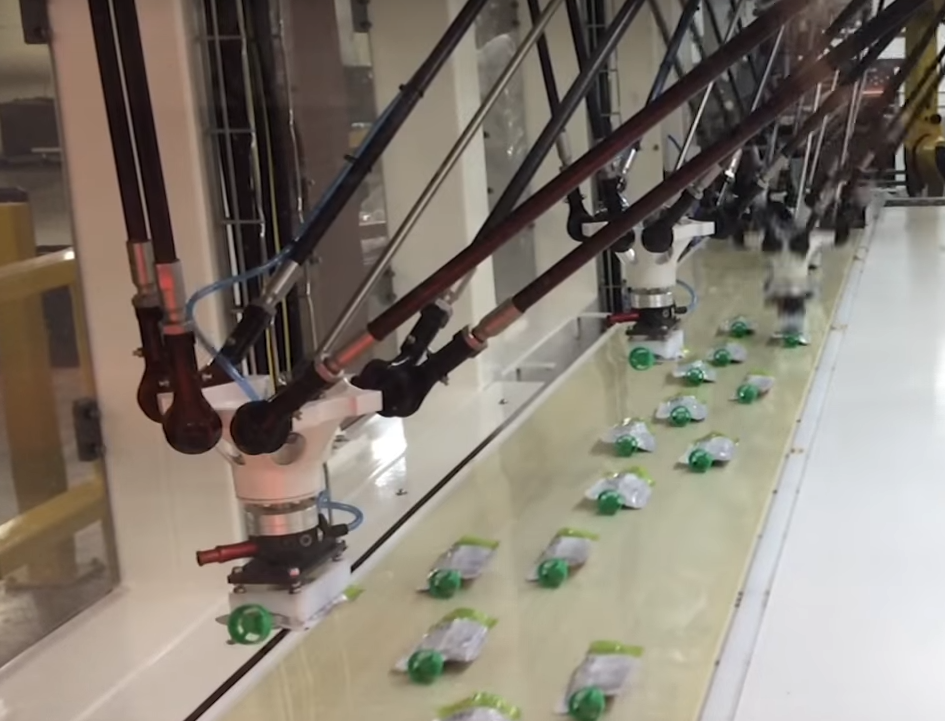
\includegraphics[width=.9\linewidth]{Applications/2022-07-18_12-59-12_screenshot.png}
\end{center}

\subsubsection{Motion simulator people}
\label{sec:org82d6322}

Easier to calculate a specific path in parallel kinematics

\href{https://www.youtube.com/watch?v=9KMptw7ZgVI\&t=1s}{Movin a dude}

\begin{center}
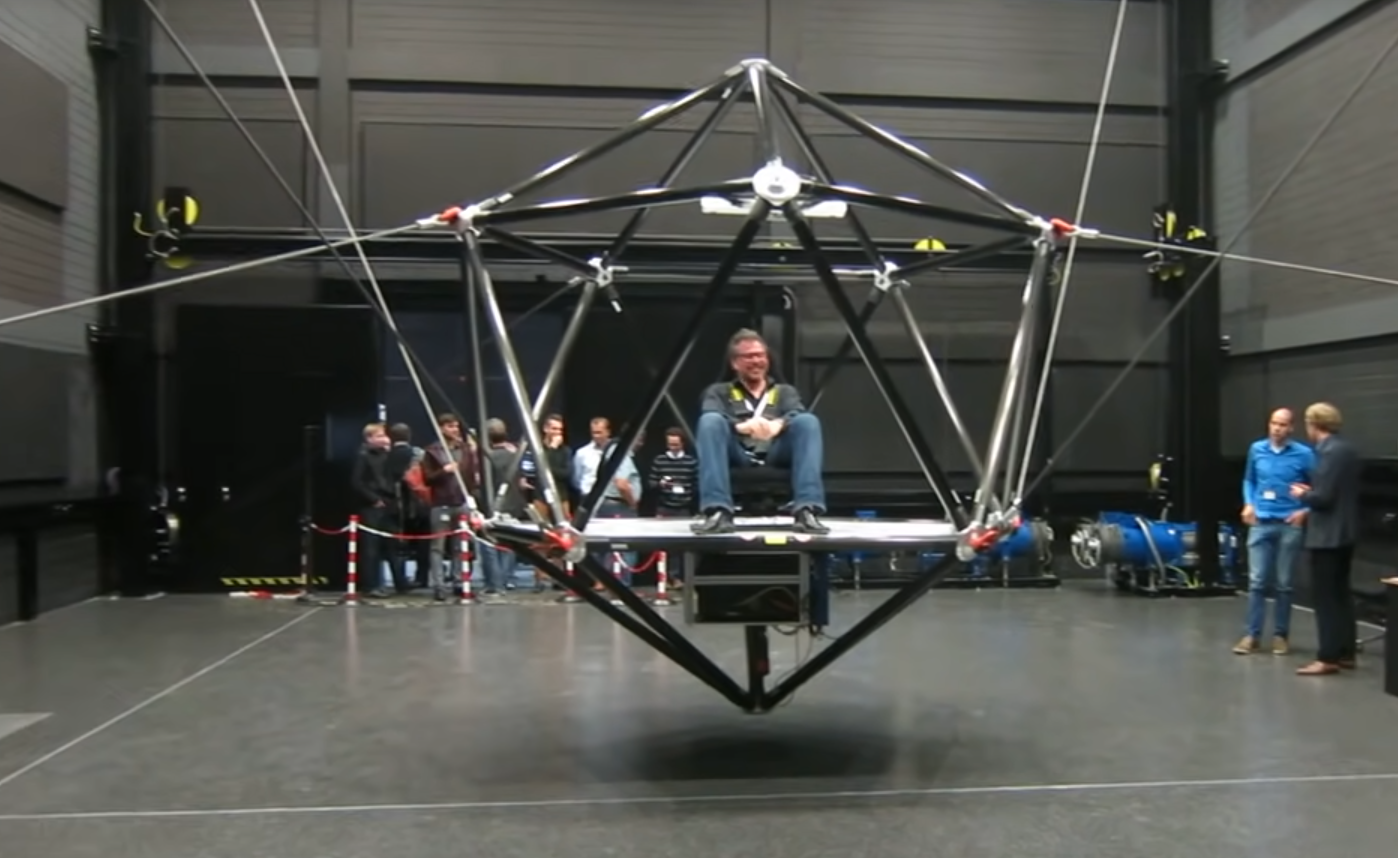
\includegraphics[width=.9\linewidth]{Applications/2022-07-18_13-03-17_screenshot.png}
\end{center}

\subsubsection{Biomedical people}
\label{sec:org8c28334}

Just trust me on this one, assaying, test verification, DNA sequencing, all automatable with parallel robotics. Bio people tend not to call it robotics though.

\subsubsection{{\bfseries\sffamily TODO} REMOVE friendly university students}
\label{sec:org0306bfc}

\url{https://ethancanderson.com/parallel-cable-robot}
\url{https://www.youtube.com/watch?v=ja98QlLI5gc}
\section{Mechanical Modules}
\label{sec:org9c7ca5d}

\subsection{Frame (8020)}
\label{sec:org3d5d1dd}

\href{https://8020.net/20-2020.html}{site}, \$0.25/inch


\subsubsection{an object}
\label{sec:orge0e219f}
\begin{center}
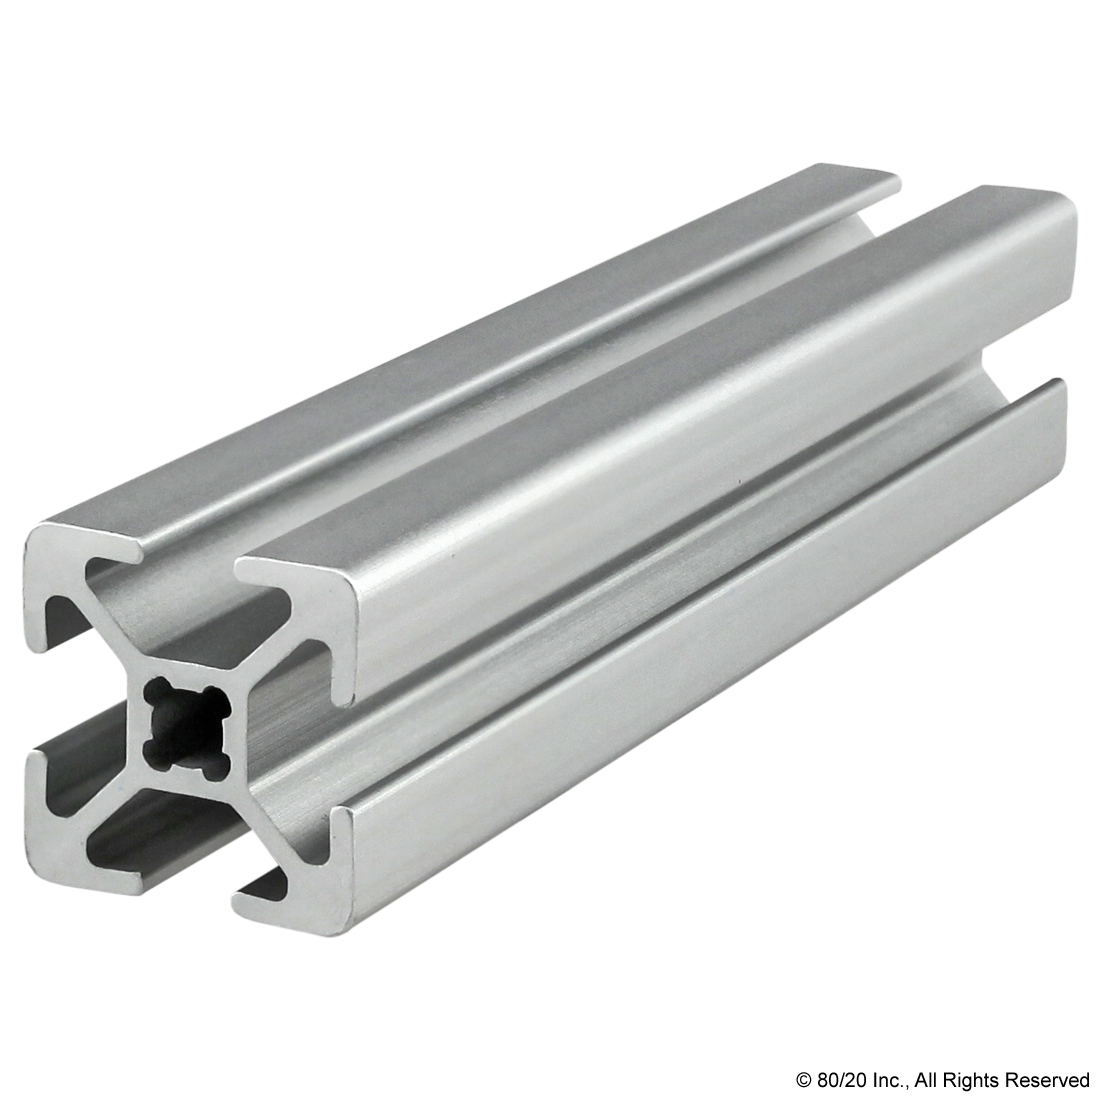
\includegraphics[width=.9\linewidth]{Hardware_needed/2022-07-18_13-11-55_screenshot.png}
\end{center}
\subsubsection{an assembly}
\label{sec:orgc86fcdd}
\begin{center}
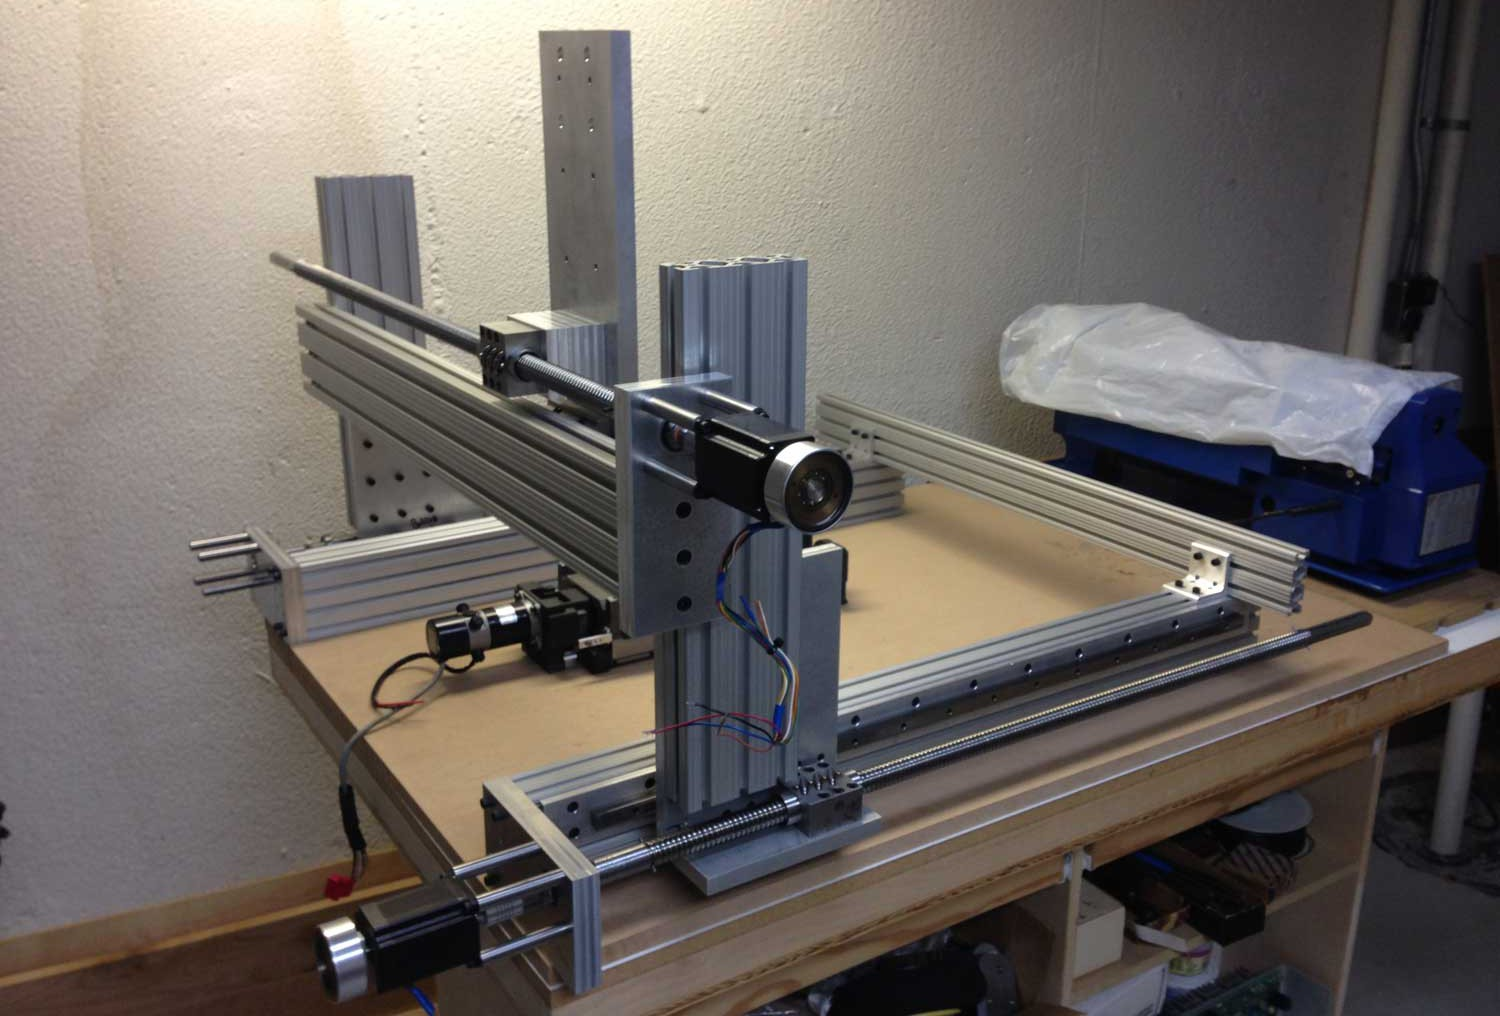
\includegraphics[width=.9\linewidth]{Hardware_needed/2022-07-18_13-13-15_screenshot.png}
\end{center}

\subsection{Effector}
\label{sec:orgeb69816}

Popular to 3d print these for passive end manipulator, probably looking at small sheetmetal project for active manipulator

\subsubsection{CoGiRo (passive)}
\label{sec:orgff5968b}
\begin{center}
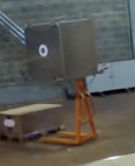
\includegraphics[width=.9\linewidth]{Hardware_needed/2022-07-18_13-31-45_screenshot.png}
\end{center}

\subsubsection{Similar Capstone (active)}
\label{sec:orgad3693d}
\begin{center}
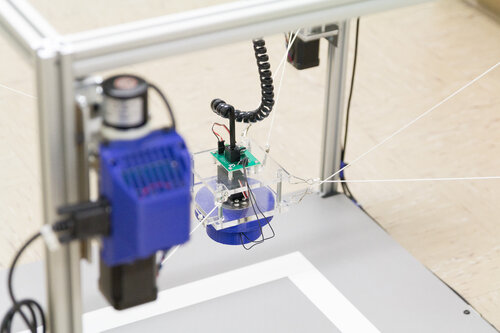
\includegraphics[width=.9\linewidth]{Hardware_needed/2022-07-18_13-32-14_screenshot.png}
\end{center}

\subsection{Winches + Pulleys (they rotate)}
\label{sec:orga222b77}

\begin{center}
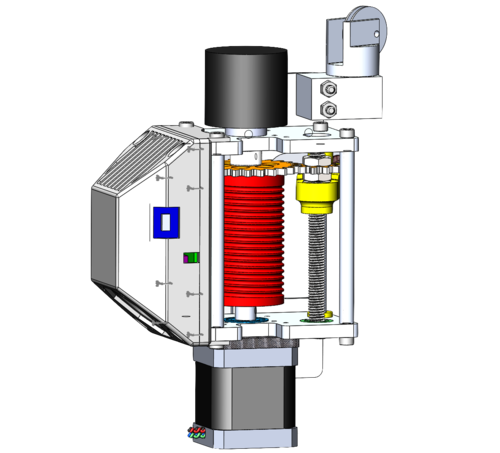
\includegraphics[width=.9\linewidth]{Hardware_needed/2022-07-18_13-16-45_screenshot.png}
\end{center}

\begin{itemize}
\item Probably looks something like that
\begin{itemize}
\item stepper motor (bottom)
\item gearing + screw (right)
\item optical encoder + PCBA for closed loop control (left)
\item pulley (top)
\item this is the mechanically challenging bit
\end{itemize}
\end{itemize}

\subsection{Stepper Motors}
\label{sec:orgf34c45d}

\href{https://www.digikey.com/en/products/compare?s=N4IgzCBcDaIEwBYCMB2ADHArCANCBAHAmAlriJgJyWZoqXkBsmBBmKKIAunglCAHoApgDsBABwBOAewAmAVwDGAFwDOAgGYBLADbKhkgav3jxBgLQBbacumT1qSgH5VAXgByCAJIBzAFYAwgBCitIAogAeSNIAIgDiAKpBlkExAILuPgBaAO4A0gCaQdIAikEoeWkARgBKQT4AEgVFlmFplmkAaj5pWQCGAWkA8gCyGX7iAdLiBNKKJWkAGiVeaQ1pAZglC1klANZpImkAUgVpKMMFPQBuPgAqaUFD7n6lABZ7e7LuIhEAYgBlLzHLR5NA9ZQxMIABTify6YGhfy8WSCflk11k0i8NQWdz6d1UOWOPjeETyCR8JQaPgOdwAXmFFASSqosmk0O5ViAAL5AA}{comparison on digikey}

Tricky to buy these guys, they tend to be expensive per unit on Digikey and I'd need to do \textasciitilde{}1 day of research into the minimum viable motor

\subsection{Mounts}
\label{sec:org73a3129}

Mounting on 8020 is super easy, literally like legos

\section{Electronics Modules}
\label{sec:orgd08b5fd}

\subsection{Effector Controller}
\label{sec:orgffa7b49}

\begin{itemize}
\item small PCBA for actuating whatever is on the effector
\item communication is possible by a trailing cable assembly or wireless
\begin{itemize}
\item cable for something requiring significant power
\item wireless for low power application
\end{itemize}
\end{itemize}

\subsection{Generic Rotary Encoder}
\label{sec:org4b67f29}

\begin{itemize}
\item You can buy these on Digikey
\item usually easy to interface them with your custom hardware (SPI/CAN/etc)
\end{itemize}

\begin{center}
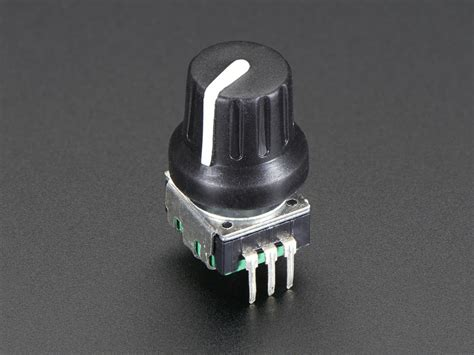
\includegraphics[width=.9\linewidth]{Electronics_Modules/2022-07-18_13-48-01_screenshot.png}
\end{center}

\subsection{Generic Stepper Motor Driver}
\label{sec:org14f281b}

\begin{itemize}
\item You can buy these on Digikey
\item Piece of hardware that generates and sends signals to our selected stepper motor
\end{itemize}

\subsection{Main Control Board}
\label{sec:org6d42eff}
handles:
\begin{itemize}
\item pathing and kinematics
\item calibration (likely by limit switch?)
\item rotary encoder info streams
\item connection to effector
\item any fancy active controls we want to implement (like robotic vision)
\end{itemize}
probably needs to be specced for running some ROS modules, MSP432 dev boards run \$50/piece, beaglebone black SBC, or EMC32 line are also good choices
\begin{center}
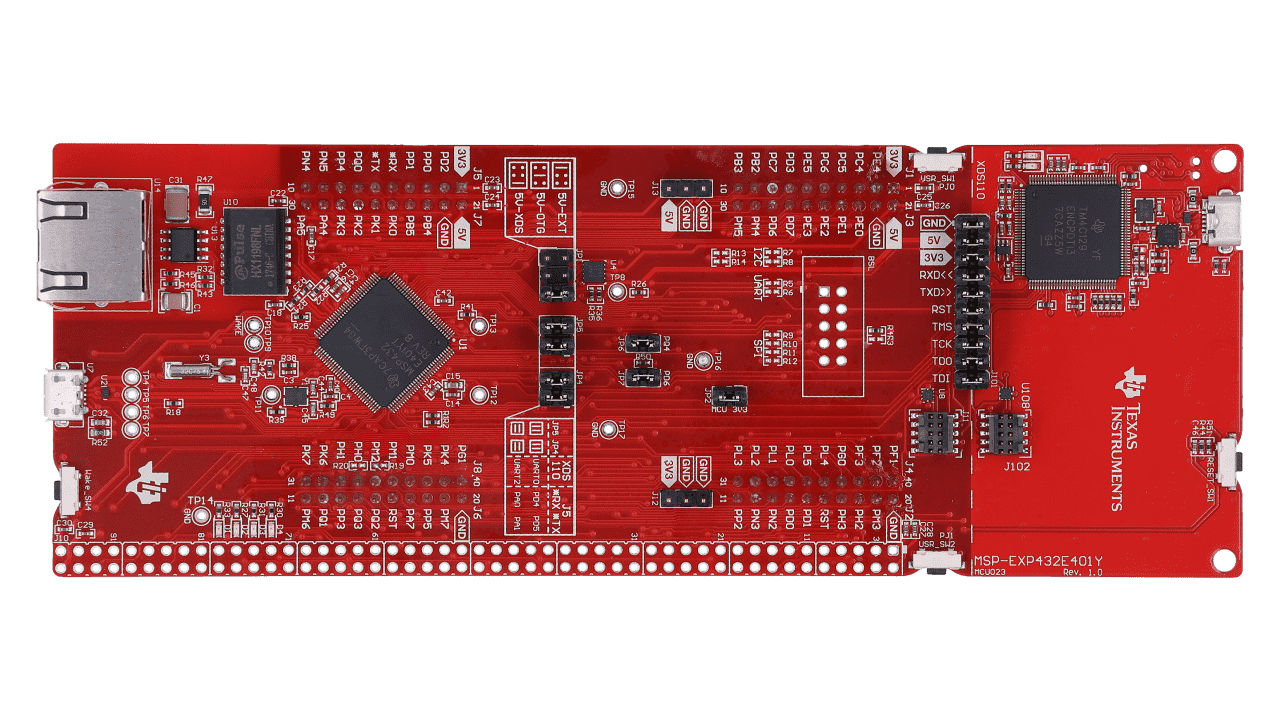
\includegraphics[width=.9\linewidth]{Main_Control_Board/2022-07-18_14-30-59_screenshot.png}
\end{center}
\begin{center}
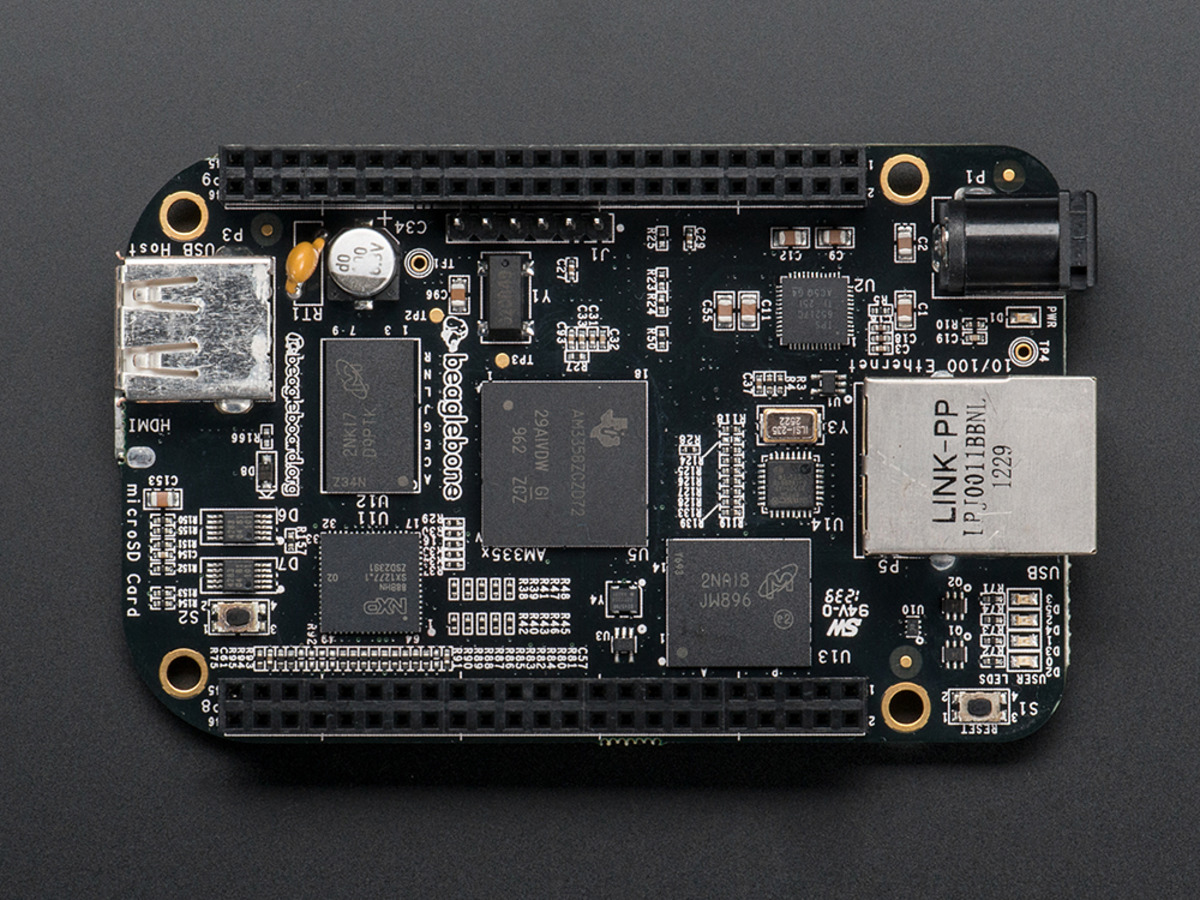
\includegraphics[width=.9\linewidth]{Main_Control_Board/2022-07-18_14-28-49_screenshot.png}
\end{center}

\subsection{Power Supply Unit}
\label{sec:orgcd363eb}
\begin{center}
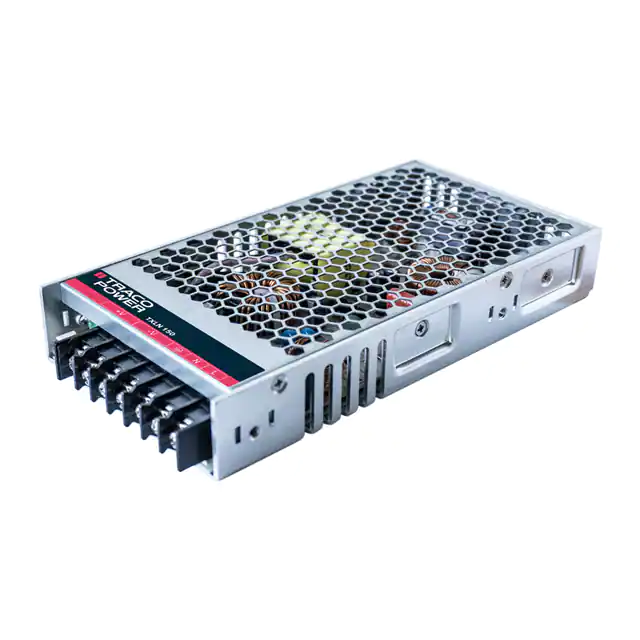
\includegraphics[width=.9\linewidth]{Power_Supply_Unit/2022-07-18_14-27-16_screenshot.png}
\end{center}
Hard to size until you know what stepper motors are drawing, what your central board is specced for, if you want to do any advanced + special control gizmos. Fermi estimate says
\begin{itemize}
\item 16 W for main board (based on beaglebone SBC max draw
\item Extremely liberal 12 W / Stepper Motor
\item Give +40\% for margin
\end{itemize}
\begin{verbatim}
SBC = 16;
SM = 12*8;
MARGIN = 1.4;
fermi_total = MARGIN * (SBC + SM)
\end{verbatim}
Tends to run \textasciitilde{}\$75/unit on Digikey, \href{https://www.digikey.com/en/products/detail/traco-power/TXLN-150-124/13681763}{link}

\section{Some Decent Whitepapers}
\label{sec:org309d56c}

\href{https://www.cambridge.org/core/services/aop-cambridge-core/content/view/B129C939BF4491AA693A36A54AE6D2C7/S0263574721001971a.pdf/full-dynamic-model-of-3-upu-translational-parallel-manipulator-for-model-based-control-schemes.pdf}{Kinematics for parallel control schemes}
\href{https://ieeexplore.ieee.org/stamp/stamp.jsp?arnumber=9737194}{on dealing with tension in large cable-driven systems}
\href{https://ieeexplore.ieee.org/stamp/stamp.jsp?arnumber=9737158}{dynamic calibration of cable-driven systems}
\href{https://arxiv.org/pdf/2003.08860.pdf}{adaptive control under uncertainty in parallel robotics}

\section{Challenges}
\label{sec:org8ac6786}

\begin{itemize}
\item Custom hardware at microcontroller level can be tricky
\item Winch design likely to involve some interaction with mechanical engineering
\item Real time kinematics calculations can be a challenging CS thing, getting to the correct O(n) is critical
\item Active position control can be mathematically involved sometimes
\item Robotics can be mathematically involved sometimes
\item Cable tension problems must be accounted for; for high speed or high robot:object mass ratios
\end{itemize}



\section{Vision Applications}
\label{sec:org105fe64}

If we feel ambitious the clear thing to do in robotics is usually to add a camera + vision daughter board, demonstrate that we can throw and catch items. I have not done vision like this, super speculative.
\end{document}